\documentclass{article}
\usepackage{amsmath}
\usepackage{amssymb}
\usepackage{amsfonts}
\usepackage{latexsym}
\usepackage{amsthm}
\usepackage[pdftex]{graphicx}
\usepackage{color}
\usepackage{xspace}
\usepackage[x11names, rgb]{xcolor}
\usepackage[utf8]{inputenc}
\usepackage{tikz}
\usepackage{dot2texi}
\usetikzlibrary{snakes,arrows,shapes}

\setlength{\topmargin}{-0.5in} \setlength{\textwidth}{6.5in}
\setlength{\oddsidemargin}{0.0in} \setlength{\textheight}{9.1in}

\newlength{\pagewidth}
\setlength{\pagewidth}{6.5in} \pagestyle{empty}

\newcommand{\R}{\mathbb{R}}
\newcommand{\N}{\mathbb{N}}
\newcommand{\Z}{\mathbb{Z}}
\newtheorem{lma}{Lemma}
\author{Chao Xu}
\title{AMS 301 Spring 2010: Homework \#2}
\date{}
\begin{document}
\maketitle
\vspace{-.5in}
\section*{Supplement II}
\subsection*{4}
$K_n$ has ${n \choose 2}$ edges. ${10 \choose 2}<50<{11 \choose 2}$. The least
number of vertices is 11.

\section*{1.3}
\subsection*{6}
Isomorphic graph have same amount of edges. Thus $G$ and $\bar G$ has the same
amount of edges. $G$ have half of the edge of $K_n$. $G$ have
$\frac{n(n-1)}{4}$ edges.

\subsection*{8}
Consider only one conference. There are 13 teams play 11 times with each other.
The sum of degrees are $143$, which is not a even number. It is not possible
for such play.

\section*{1.4}
\subsection*{3}
\paragraph*{(f)}
It can be shown that $\{d,a,h\}$ and $\{i,f,c\}$ creates $K_{3,3}$ Where
$j,b,e,g$ lies between $(a,i),(a,c),(d,f),(f,h)$ respectively.

\paragraph*{(j)}
It can be shown that $\{f,a,c\}$ and $\{b,d,g\}$ creates $K_{3,3}$.

\subsection*{4}

\begin{tikzpicture}[>=latex',line join=bevel,]
%%
\node (a) at (28bp,119bp) [draw,ellipse] {$a$};
  \node (c) at (128bp,19bp) [draw,ellipse] {$c$};
  \node (b) at (103bp,94bp) [draw,ellipse] {$b$};
  \node (e) at (53bp,94bp) [draw,ellipse] {$e$};
  \node (d) at (53bp,44bp) [draw,ellipse] {$d$};
  \node (g) at (103bp,44bp) [draw,ellipse] {$g$};
  \node (f) at (128bp,119bp) [draw,ellipse] {$f$};
  \node (h) at (28bp,19bp) [draw,ellipse] {$h$};
  \draw [] (f) -- node {$ $} (b);
  \draw [] (h) -- node {$ $} (a);
  \draw [] (c) -- node {$ $} (g);
  \draw [] (b) -- node {$ $} (g);
  \draw [] (c) -- node {$ $} (h);
  \draw [] (d) -- node {$ $} (g);
  \draw [] (a) -- node {$ $} (f);
  \draw [] (e) -- node {$ $} (d);
  \draw [] (e) -- node {$ $} (b);
  \draw [] (a) -- node {$ $} (e);
  \draw [] (h) -- node {$ $} (d);
  \draw [] (f) -- node {$ $} (c);
%
\end{tikzpicture}

\subsection*{7}
\paragraph*{(f)}
$e = 4\times 6/2 = 12$\\
$v = 4$\\
$r = 10$\\
A connected planar graph must stastify $e\leq 3v-6$\\
$12 > 3\times 4 - 6$\\
It is not a planar graph.
\paragraph*{(i)}
$r = e-v+2$\\
Each region is bounded by 4 edges. Each edge touches 2 region.\\
$r = 4/2 r - v + 2$\\
$r = 2r -v +2$\\
$r = 10$\\
$e = 20$\\
\begin{tikzpicture}[>=latex',line join=bevel,]
%%
\node (a) at (28bp,119bp) [draw,ellipse] {$ $};
  \node (c) at (128bp,19bp) [draw,ellipse] {$ $};
  \node (b) at (128bp,119bp) [draw,ellipse] {$ $};
  \node (e) at (48bp,99bp) [draw,ellipse] {$ $};
  \node (d) at (28bp,19bp) [draw,ellipse] {$ $};
  \node (g) at (108bp,39bp) [draw,ellipse] {$ $};
  \node (f) at (108bp,99bp) [draw,ellipse] {$ $};
  \node (i) at (68bp,79bp) [draw,ellipse] {$ $};
  \node (h) at (48bp,39bp) [draw,ellipse] {$ $};
  \node (k) at (88bp,59bp) [draw,ellipse] {$ $};
  \node (j) at (88bp,79bp) [draw,ellipse] {$ $};
  \node (l) at (68bp,59bp) [draw,ellipse] {$ $};
  \draw [] (j) -- node {$ $} (f);
  \draw [] (b) -- node {$ $} (c);
  \draw [] (e) -- node {$ $} (h);
  \draw [] (l) -- node {$ $} (i);
  \draw [] (f) -- node {$ $} (g);
  \draw [] (k) -- node {$ $} (g);
  \draw [] (g) -- node {$ $} (h);
  \draw [] (e) -- node {$ $} (f);
  \draw [] (j) -- node {$ $} (k);
  \draw [] (l) -- node {$ $} (h);
  \draw [] (g) -- node {$ $} (c);
  \draw [] (i) -- node {$ $} (j);
  \draw [] (d) -- node {$ $} (a);
  \draw [] (a) -- node {$ $} (e);
  \draw [] (b) -- node {$ $} (f);
  \draw [] (a) -- node {$ $} (b);
  \draw [] (i) -- node {$ $} (e);
  \draw [] (l) -- node {$ $} (k);
  \draw [] (c) -- node {$ $} (d);
  \draw [] (h) -- node {$ $} (d);
%
\end{tikzpicture}

\end{document}
\theend
